\documentclass[tikz,convert=false]{standalone}
\makeatletter
\newif\iftikz@ortho@preflush
\tikz@ortho@preflushtrue
\let\tikz@origtotarget\pgfutil@empty
\tikzset{
  |-/.style={to path={|- (\tikztotarget) \tikztonodes}},
  -|/.style={to path={-| (\tikztotarget) \tikztonodes}},
  *|/.style={to path={%
    \pgfextra
      \iftikz@shapeborder
        \tikz@scan@one@point\pgfutil@firstofone(\tikztotarget)\relax
        \ifdim\pgf@y>\tikz@lasty\relax
          \edef\tikztostart{\tikztostart.north}%
        \else
          \edef\tikztostart{\tikztostart.south}%
        \fi
      \fi
    \endpgfextra
    (\tikztostart-|\tikztotarget) -- (\tikztotarget) \tikztonodes
  }},
  *-/.style={to path={%
    \pgfextra
      \iftikz@shapeborder
        \tikz@scan@one@point\pgfutil@firstofone(\tikztotarget)\relax
        \ifdim\pgf@x>\tikz@lastx\relax
          \edef\tikztostart{\tikztostart.east}%
        \else
          \edef\tikztostart{\tikztostart.west}%
        \fi
      \fi
    \endpgfextra
    (\tikztostart|-\tikztotarget) -- (\tikztotarget) \tikztonodes
  }},
  |*/.style={to path={%
    \pgfextra
      \tikz@scan@one@point\pgfutil@firstofone(\tikztotarget)\relax
      \iftikz@shapeborder
        \let\tikz@origtotarget\tikztotarget
        \ifdim\pgf@y>\tikz@lasty\relax
          \edef\tikztotarget{\tikztotarget.south}%
        \else
          \edef\tikztotarget{\tikztotarget.north}%
        \fi
      \fi
    \endpgfextra
    (\tikztostart) -- (\tikztostart|-\tikztotarget) \tikztonodes \ifx\tikz@origtotarget\pgfutil@empty\else\iftikz@ortho@preflush(\tikz@origtotarget)\fi\fi
  }},
  -*/.style={to path={%
    \pgfextra
      \tikz@scan@one@point\pgfutil@firstofone(\tikztotarget)\relax
      \iftikz@shapeborder
        \let\tikz@origtotarget\tikztotarget
        \ifdim\pgf@x>\tikz@lastx\relax
          \edef\tikztotarget{\tikztotarget.west}%
        \else
          \edef\tikztotarget{\tikztotarget.east}%
        \fi
      \fi
    \endpgfextra
    (\tikztostart) -- (\tikztostart-|\tikztotarget) \tikztonodes \ifx\tikz@origtotarget\pgfutil@empty\else\iftikz@ortho@preflush(\tikz@origtotarget)\fi\fi
  }},
  node as new start/.is if=tikz@ortho@preflush
  }
\makeatother
\begin{document}
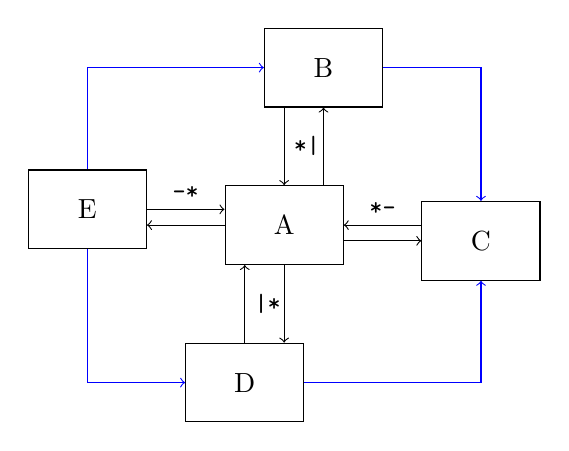
\begin{tikzpicture}
\begin{scope}[nodes={shape=rectangle, draw, minimum width=+1.5cm, minimum height=+1cm}]
  \node (a)                {A};
  \node (b) at (  .5, 2  ) {B};
  \node (c) at ( 2.5,- .2) {C};
  \node (d) at (- .5,-2  ) {D};
  \node (e) at (-2.5,  .2) {E};
\end{scope}
\tikzset{nodes={auto,font=\small\ttfamily}}
\path[->] (a) edge[*|]                 (b)
          (b) edge[*|] node {*|}       (a)
          (a) edge[*-]                 (c)
          (c) edge[*-] node[swap] {*-} (a)
          (a) edge[|*]                 (d)
          (d) edge[|*] node[swap] {|*} (a)
          (a) edge[-*]                 (e)
          (e) edge[-*] node       {-*} (a)
          %
          {[every edge/.append style=blue]
            {[|-]
              (e) edge (b)
                  edge (d)}
            {[-|]
              (b) edge (c)
              (d) edge (c)}}
;
\end{tikzpicture}
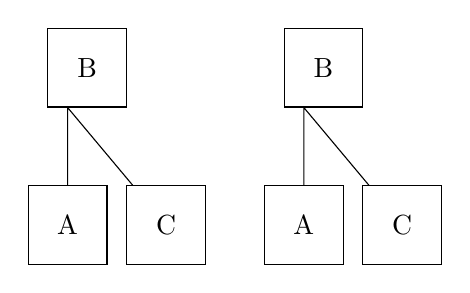
\begin{tikzpicture}[nodes={shape=rectangle, draw, minimum width=+1cm, minimum height=+1cm}]
  \node (a)              {A};
  \node (b) at ( .25, 2) {B};
  \node (c) at (1.25,-0) {C};
  \draw (a) to [|*] (b) to (c);

  \begin{scope}[xshift=3cm, node as new start=false]
    \node (a)              {A};
    \node (b) at ( .25, 2) {B};
    \node (c) at (1.25,-0) {C};
    \draw (a) to [|*] (b) to (c);
  \end{scope}
\end{tikzpicture}
\begin{tikzpicture}[nodes={rectangle,draw,anchor=west,minimum height=+1cm}]
\node (rechteck1)[minimum width=+3cm] at (1,5){};
\node (rechteck2)[minimum width=+2cm] at (1,3){};

\draw [->] (rechteck1) to[*|] (rechteck2);
\end{tikzpicture}
\end{document}